\documentclass[modern]{aastex62}
\begin{document}

\title{The Leaky Pipeline for Postdocs: A study of the time to reach a faculty job for male and female astronomers}
\correspondingauthor{Kevin Flaherty}
\email{kevin.flaherty@williams.edu}

\author[0000-0003-2657-1314]{Kevin Flaherty}
\affil{Van Vleck Observatory, Astronomy Department, Wesleyan University \\
96 Foss Hill Drive \\
Middletown, CT 06459, USA}
\affil{Department of Astronomy, Williams College \\
Williamstown, MA 01267, USA}

\begin{abstract}
The transition between receiving a PhD and securing a tenure track faculty position, for those interested in working in academia, is challenging for all astronomers. Young scientists typically spend anywhere between 1 and 10 years (or more)  publishing as many papers as possible, building collaborations, traveling to conferences, gaining experience in advising, teaching, and new instruments/software, all while moving between multiple institutions and spending a substantial amount of time on job applications. Here we use a publicly available database of recently hired faculty to examine the amount of time astronomers typically spend in this transitory state. We find that the average time spent between receiving a PhD and being hired into a faculty position is 4.9$\pm$0.3 years, with female astronomers hired on average 4.2$\pm$0.4 years after receiving a PhD and male astronomers typically hired after 5.3$\pm$0.4 years. We examine a number of models to explain this gendered effect, and rule out the increase in women receiving a PhD in recent years, as well as a bias in favor of hiring women into faculty positions. The most likely model is one in female astronomers leave the academic job market at a $\sim$3 times higher rate than male astronomers. This is another sign of the leaky pipeline, and indicates that more work can be done to retain female astronomers during the postdoc stage of their career.
\end{abstract}


\section{Introduction}

Across many of the factors that would make a faculty candidate appealing to a hiring committee, many studies have shown a persistent bias in favor of male scientists. Men are invited to give more colloquia than women (nittrouer et al. 2017), have a higher success rate at receiving telescope time (lonsdale et al. 2016, reid 2014, patat 2016, spekkens et al. 2018), are cited more frequently (caplar et al. 2017), ask more questions at conferences (schmidt \& davenport 2017, schmidt et al. 2017, davenport et al. 2014, pritchard et al. 2014, hinsley et al. 2017), are overrepresented among prestigious physics fellowships (nordstrom et al. 2018), and have their abstracts rated at a higher level of scientific quality (knobloch-westerwick et al. 2013). These biases exist despite the lack of evidence for biological differences in science and math ability (giglio 2017, ref). Elite male faculty in the life sciences are less likely to take on female students (sheltzer \& smith 2014), limiting early entry points into the field, and recommendation letters show gender-based biases (dutt et al. 2016).  Female scientists that are able to navigate these effects still have to deal with high rates of sexual harassment (clancy et al. 2014, national academies study), and higher demands on their time (el-alayli et al. 2018). These factors can lead to a female candidate appearing less qualified than an otherwise equivalent male candidate. 

Even among candidates with identical qualifications there is a bias against women. moss-racusin et al. 2012 found that identical resumes were graded differently based on the gender of the applicant; women were offered a lower salary and were less likely to be offered a position. More reservations are expressed about CVs from female faculty members (stenpreis et al. 1999), and in hiring decisions relationship more often discussed, always as a negative, for female faculty candidates (rivera 2017). 

Hiring biases based on race/ethnicity are also present (gibbs et al. 2016, betrand \& mullainathan 2004), but have been studied much less frequently in part due the lack of a large enough sample within many STEM fields. To our knowledge no study has been done on the hiring of individuals with a non-binary gender, or of individuals who identify as LGBTQ. {\it Mention the results of studies on the working conditions for LGBTQ scientists, since that will affect how long someone stays within the field.}

Biases against hiring women can change the length of time it takes to transition from getting a PhD into a tenure-track faculty position. Conversely, a push towards hiring women, in an effort to increase the diversity of the faculty ranks, may lead to women being hired more quickly out of graduate school. Here we examine the time between when an astronomer receives a PhD and when they are hired into a tenure track faculty position, using a publicly available listing of recent faculty hires. In section~\ref{data} we discuss the data collection, and the average hiring time for male and female astronomers. In section~\ref{model} we introduce a model for the labor market, including gendered effects that may potentially explain the 

\section{Data Collection and Results\label{data}}

\subsection{Data}
The sample for this study is drawn from the Astrophysics Rumor Mill\footnote{\url{http://www.astrobetter.com/wiki/Rumor+Mill+Faculty-Staff}}. This page contains a public wiki listing various job postings within astronomy, and is updated by astronomers during the job season to indicate e.g. when phone interviews are conducted, who is on the short list, and the name of someone that has accepted the position, if any of this information is known for a particular job. 

For the purposes of this study, it serves as a public listing of astronomers that have recently been hired into tenure-track faculty positions, with information on the year in which they were hired. While this is not a complete listing of everyone that has been hired into astronomy, it can serve as a representative listing. For each rumor of an accepted job offer, which was subsequently confirmed through a Google search, we record the gender of the astronomer, the year that they were hired, the year they received a PhD, and whether they were hired by an R1 school or non-R1 school. The PhD year was detected based on a Google search for a CV, or other public listing of a graduation year, while the year that someone was hired was taken as the spring year of the hiring cycle (ie. for someone listed on the 2014-2015 rumor mill, we use 2015 as the year they were hired). We assume a gender binary (either male or female), based on information from a Google search (e.g. a picture, gendered pronouns, etc.). Data collection starts with the 2010-2011 job cycle and runs through the 2016-2017 cycle. 

We exclude astronomers that are moving between tenure-track positions since our research question is focused on the initial hiring decision. We also exclude anyone that received a PhD prior to 2000 since most of these astronomers in this range have spent a substantial amount of time working at a national lab (e.g. JPL, STSCI) before taking the tenure-track faculty position. We also focus on colleges and universities in the US since hiring practices and job responsibilities can vary substantially between US and non-US institutions. Given the very small number statistics, we do not record race/ethnicity. From this list we exclude anyone for which we could not determine the gender or the year that they received their PhD. The Carnegie classification of the hiring institution is determined using the online lookup tool\footnote{\url{http://carnegieclassifications.iu.edu/lookup/lookup.php}}, and we only record if the institution is listed as R1 (Doctoral Universities - Highest research activity) or non-R1 (including institutions that award masters degrees, as well as undergraduate only institutions). 

This leaves a total sample of 245 astronomers, 157 of which are men and 88 of which are women. The fraction of women within our sample (35$\pm$4\%) is slightly higher than the fraction of female assistant professors in 2013 (26$\pm$4\%, Hughes et al. 2014) suggesting that our sample is over-represented in terms of female astronomers. As discussed below, this slight bias is likely to be responsible for the large discrepancy in hiring time between male and female astronomers. We do not find a significant difference in the hiring time from one job cycle to the next, and consider the entire sample as a whole in order to minimize Poisson errors. 

\subsection{Results}
Figure~\ref{hiring_time} shows the distribution of time between receiving a PhD and being hired into a tenure track faculty position based on our sample. We find that, on average, astronomers spend 4.9$\pm$0.3 years in postdoc positions before being hired. Note that we only record when someone is hired, and not when they actually start their faculty job. Astronomers hired very soon out of graduate school may defer the start of their faculty position for a year or two, and our measured mean hiring time is likely a lower limit on the average time astronomers spend as a postdoc. We do not find any significant difference in the hiring time between astronomers hired into R1 institutions and non-R1 institutions (Figure~\ref{hiring_time}). We do find a significant drop in the number of astronomers hired into R1 institutions between the fifth and sixth year out of graduate school, although the origin of this drop is unclear. 

\begin{figure}[!htb]
\center
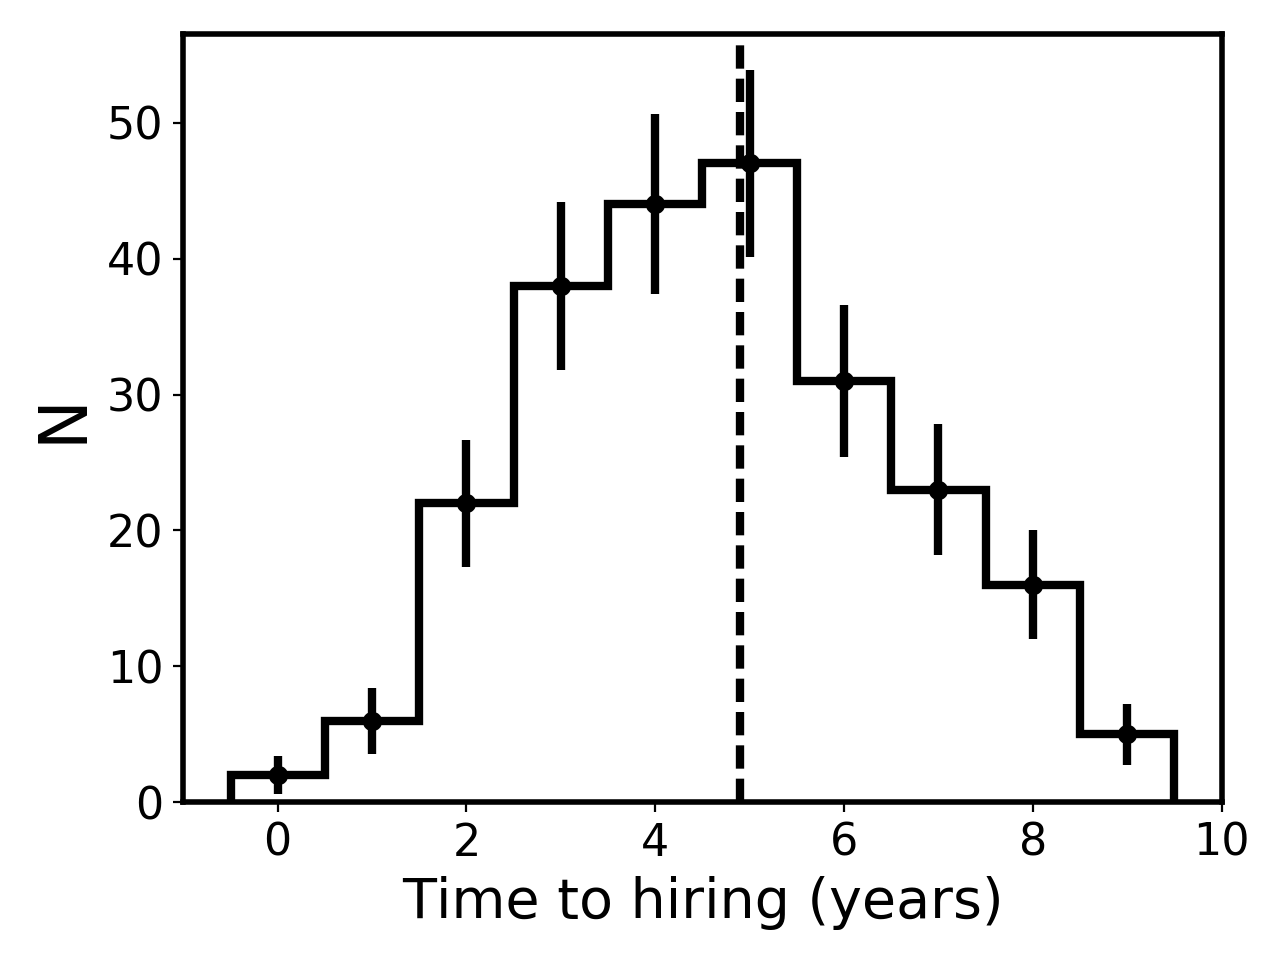
\includegraphics[scale=.3]{full_hiring_time.png}
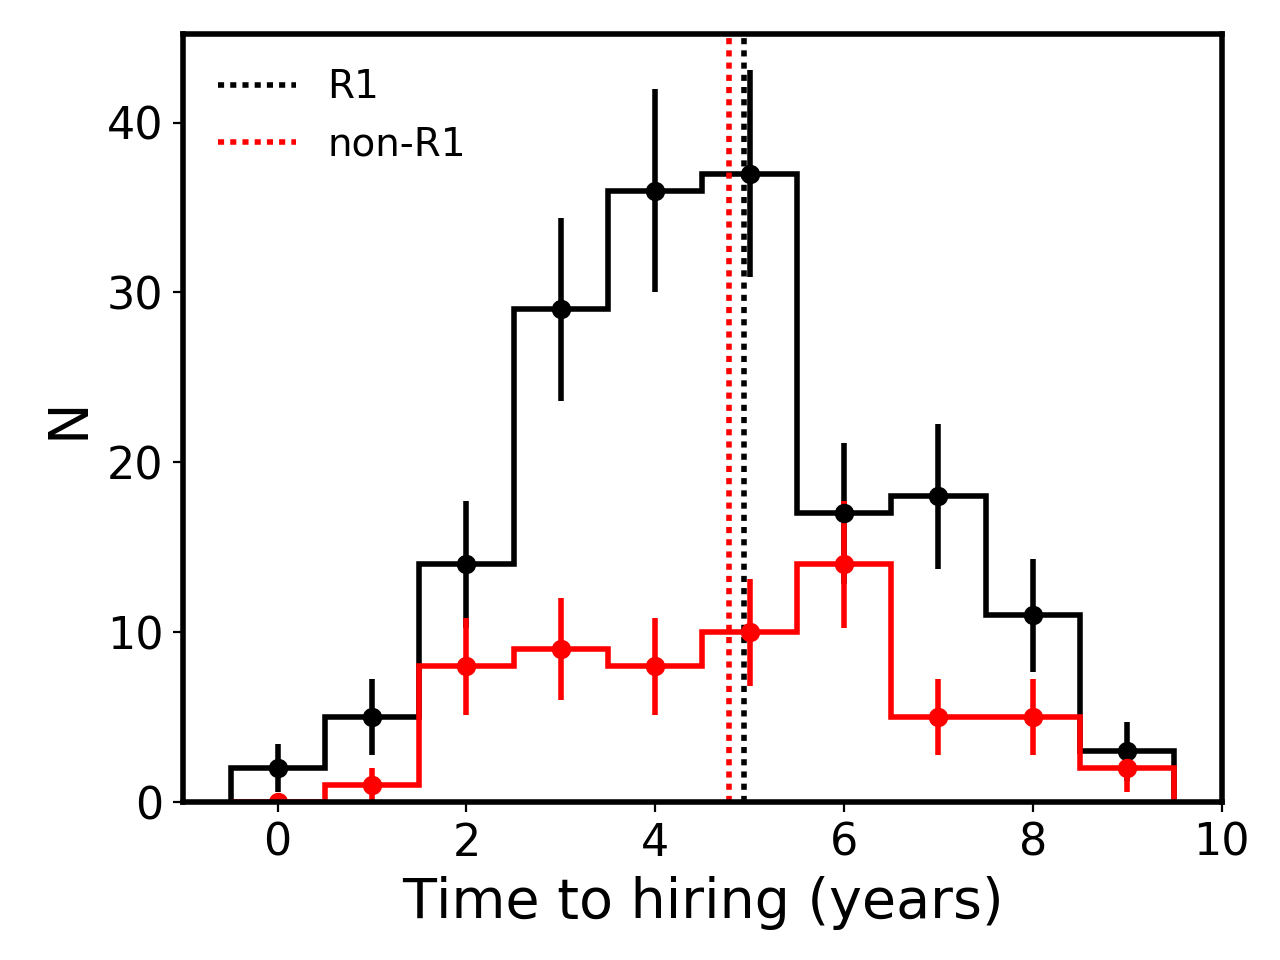
\includegraphics[scale=.3]{cc_hiring_time.png}
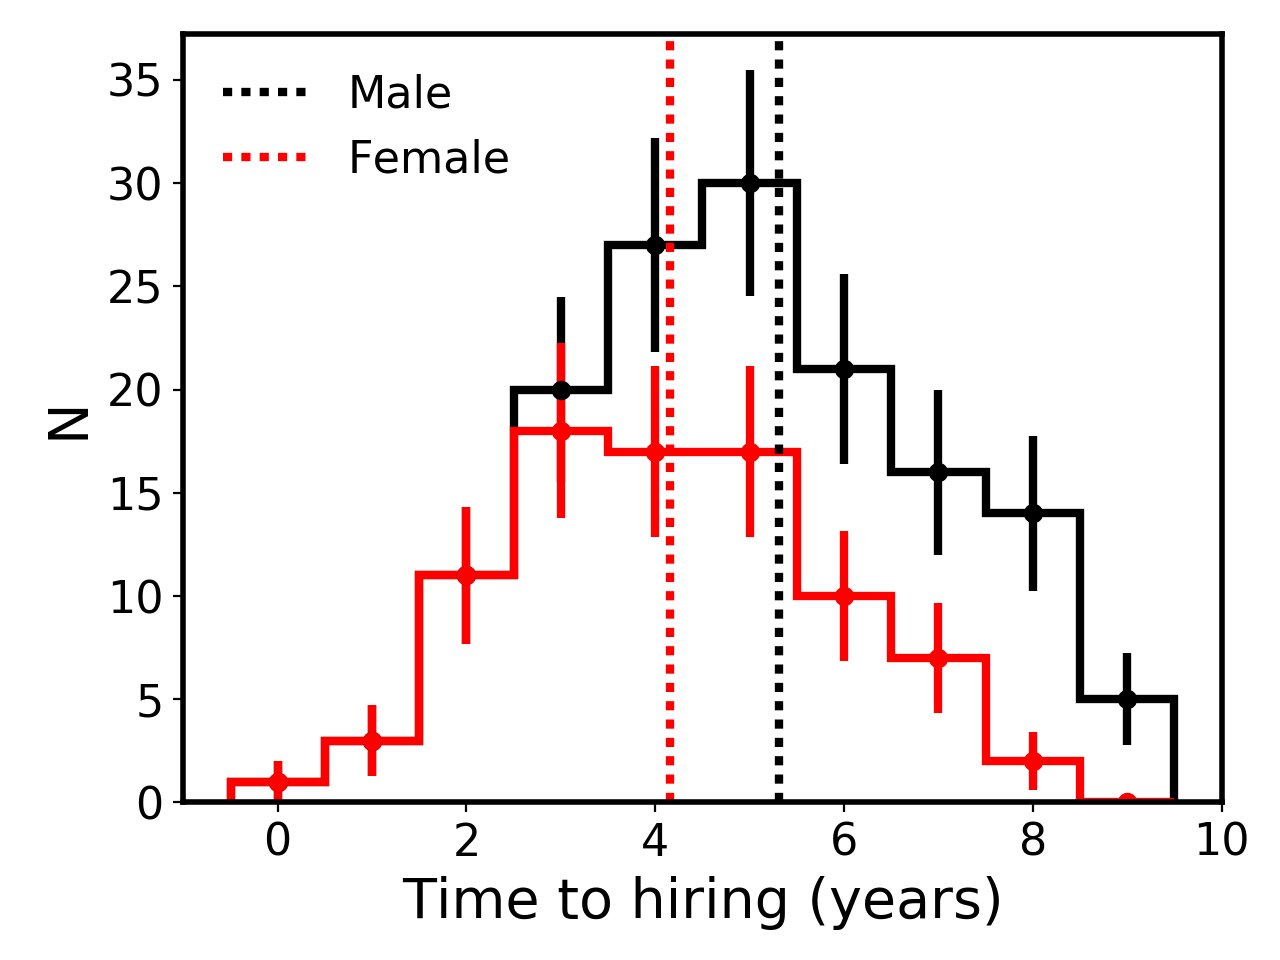
\includegraphics[scale=.3]{gender_hiring_time.png}
\caption{(Left:) Number of astronomers hired into tenure track faculty positions, as a function of time since receiving their PhD. On average astronomers spend 4.9$\pm$0.3 years in a postdoc position. (Center:) We do not find any significant difference in the hiring time for astronomers hired into R1 schools (black line) versus astronomers hired into non-R1 schools (red line). The origin of the sudden drop in the number of astronomers hired by R1 universities six years out of graduate school is unclear. (Right:) Number of male (black line) and female (red line) astronomers hired into tenure track faculty positions, as a function of time since receiving their PhD. Among our sample, an equal number of male and female astronomers are hired in the first two years out of graduate school, while twice as many male astronomers as female astronomers are hired in years 4 through 10. This leads to female astronomers being hired, on average, one year earlier than male astronomers (4.2$\pm$0.4 vs 5.3$\pm$0.4).\label{hiring_time}}
\end{figure}

Figure~\ref{hiring_time} also shows the hiring time split based on gender. We find a significant difference in how long it takes male and female astronomers to be hired into tenure track positions, with a KS probability of these two distributions being drawn from the same population of 0.03. Female astronomers are hired on average 4.2$\pm$0.4 years after receiving their PhD, while for male astronomers the average hiring time is 5.3$\pm$0.4 years. This difference is due to a substantial difference in the shape of the hiring time distributions. Within the first two years out of graduate school, the number of male and female astronomers is identical, while from years four through ten twice as many male astronomers as female astronomers are hired. Note that women are slightly over-represented in this sample, indicating that {\it at least} twice as many male astronomers as female astronomers are hired in years four through ten, and {\it at most} the number of female astronomers hired in the first two years out of graduate school is equal to the number of male astronomers hired. There is no significant evidence that the hiring time difference between male and female astronomers depends on the Carnegie classification of the hiring institution, although the small number of astronomers hired by non-R1 schools limits this conclusion. We do find that among R1 hires 68$\pm$6\% (124 out of 182) are male, while among non-R1 hires 52$\pm$19\% (33 out of 63) are male.




\section{Faculty Hiring Model\label{model}}
To understand the source of the discrepancy between when male and female astronomers are hired into tenure track faculty positions, we create a model of the hiring process, while introducing gendered factors in an attempt to reproduce both the male and female hiring time distribution.

The basic model consists of $N_{\rm phd}$ astronomers added to the labor pool, and $N_{\rm hire}$ astronomers randomly selected from the full labor market and 'hired' into a faculty position. Once an astronomer has been hired they are removed from the labor market, and the model proceeds to the next year adding another $N_{\rm phd}$ astronomers to the labor pool and removing another $N_{\rm hire}$ astronomers from the labor pool. Whenever someone is hired we record the year they were hired, the year they received their PhD, and their gender. Unless otherwise specified, we assume that 30\% of the $N_{\rm phd}$ astronomers receiving a PhD and entering the labor market are female. 

To reproduce the non-uniform hiring time distribution we assume that the probability of being hired ($p_{\rm hire}$) depends on time since the astronomer received their PhD ($t_{\rm hire}$). For $t_{\rm hire}>10$ years we assume $p_{\rm hire}$=0, while the probabilities for $t_{\rm phd}<10$ are manually adjusted. The adjustment is done to reproduce the hiring time distribution for male astronomers, while the specific model parameters are adjusted to reproduce the hiring time distribution for female astronomers. 

The labor pool is populated starting in 1980, while hiring begins in 1990. As with the data, we only consider astronomers that were hired between 2011 and 2018. The model is started well before these dates to ensure that it has reached a steady state before comparing with the data.

To avoid large statistical noise in the model, we use values of $N_{\rm phd}$ and N$_{\rm hire}$ that are much larger than reality, but still preserve the ratio of tenure track jobs to PhD astronomers. mulvey \& nicholson (2014) reports $\sim$150 PhDs rewarded from 2007 to 2012, after averaging $\sim$110 in the prior decade\footnote{AIP maintains enrollment and degree records going back to 1978 \url{https://www.aip.org/statistics/rosters/astronomy}}, while in the Astrophysics Rumor Mill there are roughly 50 tenure track faculty positions listed each year. In the model we use $N_{\rm phd}$=30000 and $N_{\rm hire}$ = 10000, consistent with the 3:1 ratio of PhDs awarded to faculty jobs available each year. This is likely an over-estimate of the $N_{\rm phd}$/$N_{\rm hire}$ ratio since we do not account for non-US astronomers that apply to US faculty jobs, and some of the US faculty positions listed on the Astrophysics Rumor Mill are for physics positions for which an astronomer is not hired. Our results will not be strongly affected by this discrepancy, unless $N_{\rm phd}\sim N_{\rm hire}$ which is highly unlikely. 

Below we consider three different explanations for the gendered hiring time distribution: (1) An increase in the number of women receiving astronomy PhDs over time, (2) A higher probability of a female astronomer being hired relative to a male astronomer, (3) Women leaving the labor market at a higher rate than male astronomers. To asses the viability of any of these models we compare the relative fraction of male and female astronomers hired in a given year with the data assembled from the rumor mill. 

We also compare our model predictions with the general demographics of the labor market. Specifically we compare to the fraction of female PhD students in 2003 (30$\pm$2\%) and the fraction of female assistant professors in 2013 (26$\pm$4\%) as measured by hughes et al. 2014, and the fraction of women in the applicant pool of tenure track faculty positions (19$\pm$3\%, thompson 2015). To calculate the number of female PhD students in 2003 we count all entries that received a PhD between 2003 and 2010. This range of times encompasses first and recently graduated students, assuming a typical PhD length of 7 years. To calculate the fraction of female assistant professors in 2013, we calculate the fraction of women among astronomers hired between 2007 and 2013. This assumes a typical time to tenure, and promotion from assistant to associate faculty) of six years. To compare with the findings of thompson 2015 we calculate the fraction of women within the labor pool in 2014. 

\subsection{Increasing Female Demographics}
The first model we consider is one in which the fraction of women within astronomy increases with time. Between 1992 and 2013 the fraction of female graduate students rose from 22\% to 34\%, while the fraction of female assistant professors increased from 17\% to 26\% over the same period (hughes et al. 2014). Adding substantially more young women to the labor pool will bias the hiring time distribution towards shorter times given that there are simply more women available to be hired.

We model the change in the fraction of women being awarded a PhD as a logistic function
\begin{equation}
f_{\rm phd} = \frac{1}{1+\exp (-s(t-t_0))}\\
\end{equation}
where $s$ controls the rate of increase in the fraction of women, $t_0$ is the year in which gender parity is reached, and $t$ is the year. We find that $s$=0.027 and $t_0$=2040 provide a reasonable fit to the demographics survey of hughes et al. 2014 (Figure~\ref{f_phd}).

\begin{figure}[!hbt]
\center
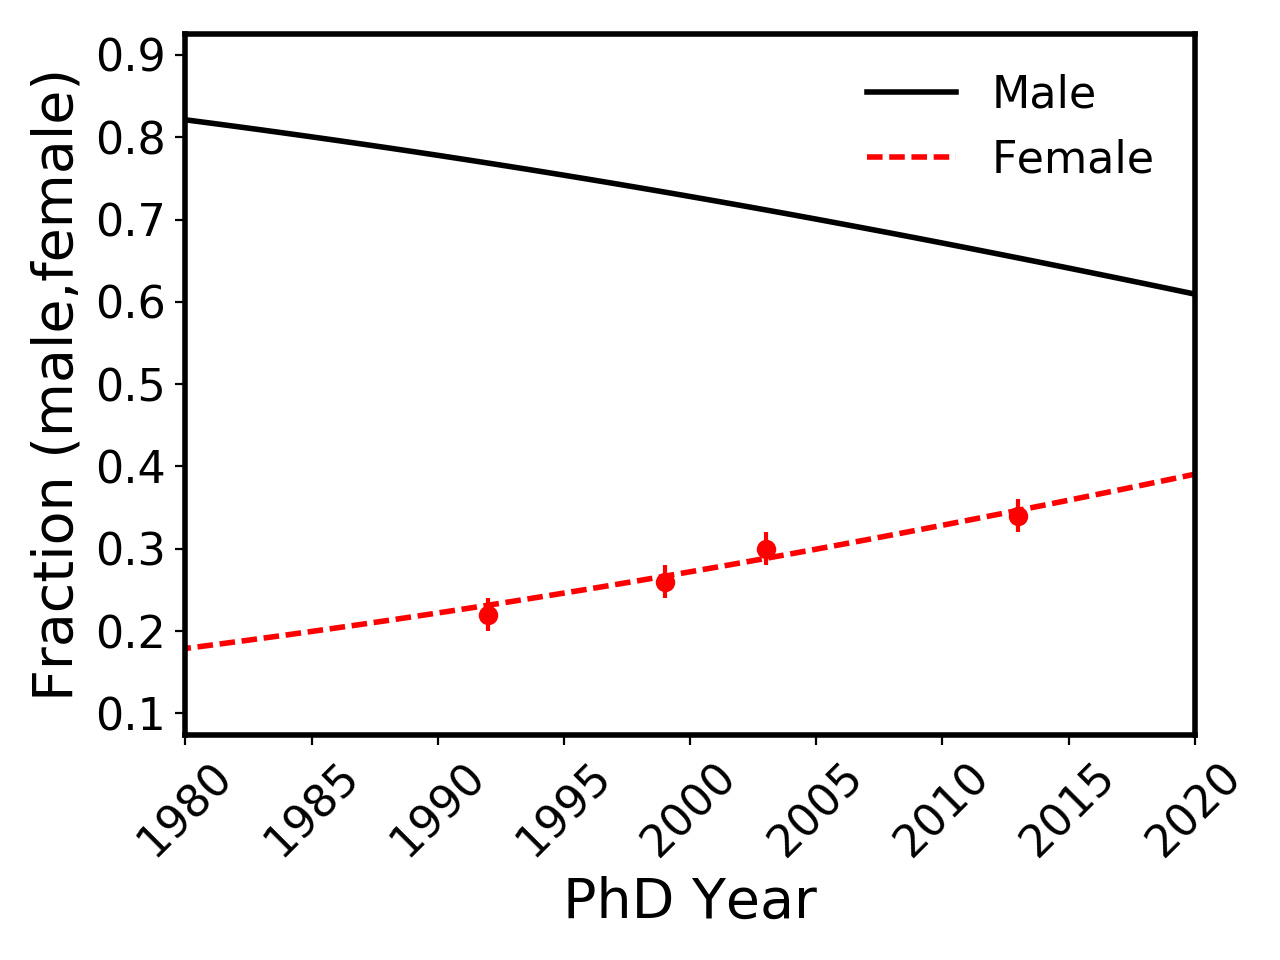
\includegraphics[scale=.6]{f_phd.png}
\caption{Fraction of male (black line) and female (red dashed line) astronomer receiving a PhD as a function of time as predicted by our model prescription, compared to the measurements of hughes et al. (2014) (red points).\label{f_phd}}
\end{figure}

Figure~\ref{model1} shows the results of this model. While this model is able to reproduce the fraction of female assistant professors in 2013 (28\% vs 26$\pm$4\%) it overpredicts the fraction of women in the labor market (24\% vs 19$\pm$3\%) and does not match the hiring time distribution for female astronomers. The increase in female astronomers is not dramatic enough to substantially tilt the hiring times of female astronomers to shorter values. 

\begin{figure}[!hbt]
\center
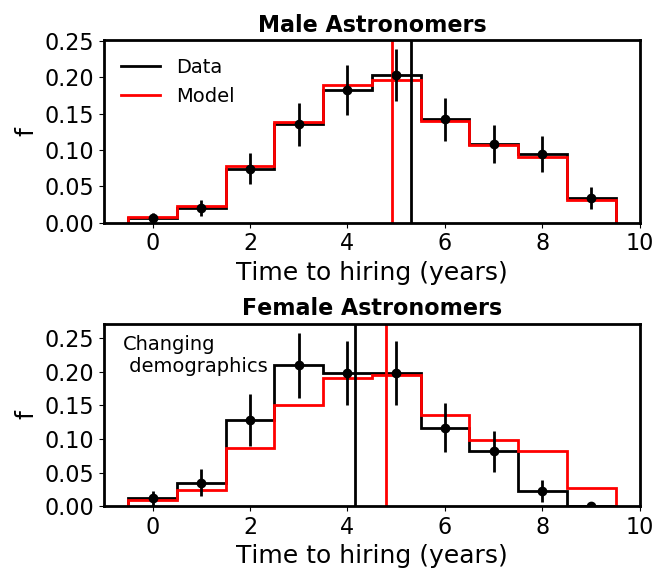
\includegraphics[scale=.6]{model1.png}
\caption{Normalized hiring time distributions for male (top panel) and female (bottom panel) astronomers. Here we include an increase in the fraction of female astronomers with time, and find that this is unable to match the hiring time distribution for female astronomers. This indicates that the increase in female astronomers is not responsible for the different hiring time distributions. \label{model1}}
\end{figure}
 

\subsection{Bias Toward Hiring Women}
In our second model, we consider a bias towards hiring women. This may occur as a result of diversity efforts leading more colleges and universities to hire women more quickly out of graduate school, or because women are intrinsically better qualified for faculty jobs. Given the finite number of women in the labor market, by quickly removing women there will be fewer female astronomers available at later times, shifting the peak of the hiring distribution towards shorter timescales.

We model a bias towards female astronomers by introducing a parameter $b$ that is a multiplicative increase in the probability of hiring a women relative to hiring a male astronomer (e.g. $b=2$ indicates that a female astronomer is twice as likely to be hired as a male astronomer). This multiplicative factor is applied to all female astronomers regardless of when they receive their PhD. 

\begin{figure}[!hbt]
\center
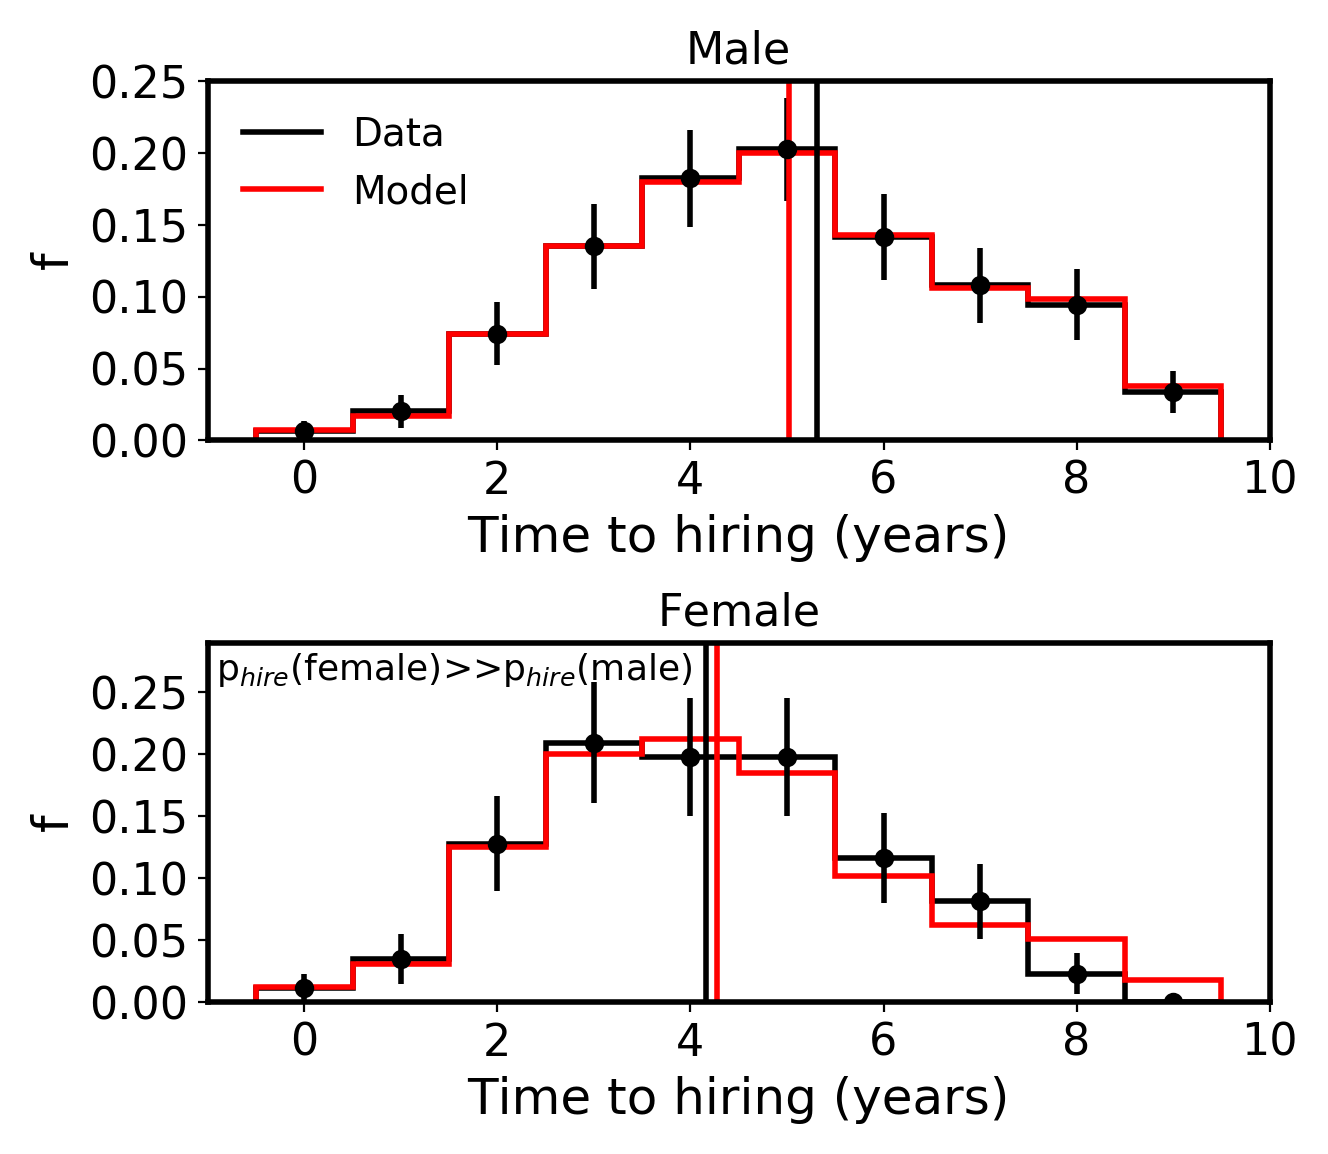
\includegraphics[scale=.6]{model2_b10.png}
\caption{Normalized hiring time distributions for male (top panel) and female (bottom panel) astronomers. Here we introduce a bias in favor of hiring women. While this is able to match the normalized hiring time distribution for women, it requires that a female astronomer is 10 times more likely to be hired into a faculty position. This model predicts that 70\%\ of assistant professors in 2013, which is much larger than the measured value (26$\pm$4\%). \label{model2_b10}}
\end{figure}

We are able to reproduce the normalized hiring time distribution for female astronomers (Figure~\ref{model2_b10}), but only with $b=10$. It is highly unlikely that a female astronomer is 10 times more likely to be hired than a male astronomer, especially given that this predicts that 70\%\ of assistant professors in 2013 are female, when in reality only 26$\pm$4\% are female. 

The need for a strong bias in this scenario is because the number of PhDs produced each year far outnumbers the number of tenure track faculty jobs available, even without accounting for non-US PhD students entering the US labor market (which will increase $N_{\rm phd}$), or the presence of physics positions on the the rumor mill (which will reduce $N_{\rm hire}$). Under these conditions it takes a substantial bias in favor of women in order for the number of female astronomers hired each year to substantially deplete the labor market. hughes et al. 2014 find that only $\sim$15\% of graduate students from 2003 make it into faculty positions in 2013, consistent with a saturation of the faculty labor market. Our model result indicates that there is no evidence for a bias in favor of hiring women 

\subsection{Women Leaving the Labor Market}
The third model we consider is one in which astronomers leave the labor pool at a rate that increase with time. There are many factors that can drive someone out of the academic job market, including the low probability of landing a position as discussed above, and these factors may vary between male and female astronomers.

To model this effect we introduce an exponential function that defines the fraction of the astronomers leaving the labor market as a function of time since receiving a PhD.
\begin{equation}
f_{\rm leave} = 1-\exp (t-2/\tau).
\end{equation}
We assume that no one leaves until two years after receiving a PhD, and that the shape of the subsequent function is defined by the variable $\tau$. A smaller $\tau$ implies that the fraction of astronomers leaving the faculty labor market increases rapidly with time, while a larger $\tau$ results in a smaller fraction of astronomers leaving the labor market. Female and male astronomers have different values of $\tau$ to allow for different departure rates for male and female astronomers. 

\begin{figure}[!hbt]
\center
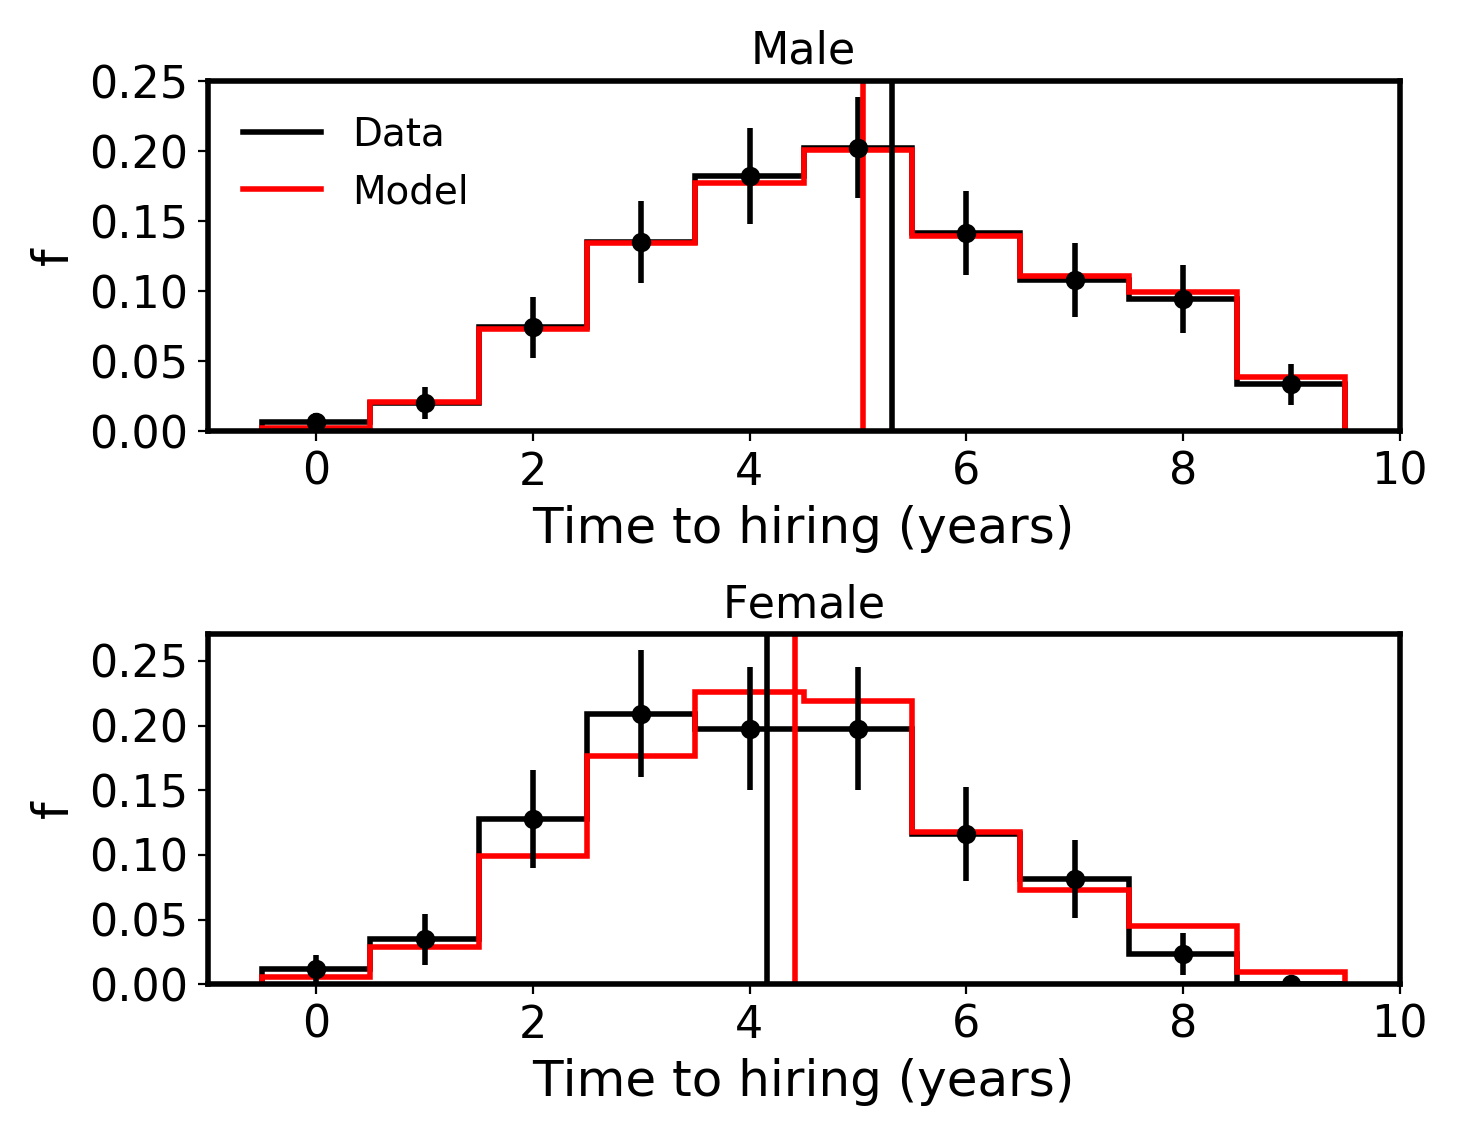
\includegraphics[scale=.6]{model3.png}
\caption{Normalized hiring time distributions for male (top panel) and female (bottom panel) astronomers. Here a fraction of astronomers leave the labor market every year, starting the second year out of graduate school. By introducing a higher rate of departure for female astronomers, we are able to reproduce the normalized hiring time distribution for female astronomers. This models also predicts that women make up 18\%\ of the labor market and 24\% of assistant professors in 2013, similar to the measured fractions (19$\pm$3\% and 26$\pm$4\% respectively).  \label{model3}}
\end{figure}

This model is able to produce a reasonable match to the normalized hiring time distribution for female astronomers with $\tau_{\rm male}$=40 and $\tau_{\rm female}$=10. It also predicts that women make up 18\% of the labor market and 24\% of assistant professors in 2013, consistent with the measured values of 19$\pm$3\% (thompson 2015) and 26$\pm$4\% (hughes et al. 2014) respectively. Within this model the fraction of women leaving the labor market is 3-4 times higher than the fraction of men leaving the labor market. Given the relative proportion of female and male astronomers entering the labor market, this means that, in terms of total number, as many female astronomers (if not more) leave the academic labor market as male astronomers, despite the fact that male astronomers strongly outnumber female astronomers. 

\subsubsection{Long Term Demographics}
With a successful predictive model, we can predict the future increase in women with time, and by extending the model into the past we can predict the fraction of female associate and full professors. In this way we can examine whether or not a substantial fraction of female astronomers leave academia after securing a tenure track faculty position. 

\section{Conclusions}

\acknowledgements
I want to thank the Wesleyan STEM Diversity Journal Club for their thoughts about the results, and for providing an opportunity to discuss these issues among a supportive group.

\begin{thebibliography}{}

\end{thebibliography}


\end{document}
